\section{Methods} \label{sec:methods}

It is necessary to optimize reconstruction to get high quality results with tractable genome sizes and limit the impact on memory usage and bandwidth usage.
Hereditary stratigraphy \citep{moreno2022hereditary} was designed to do this.

We have successfully demonstrated aspects of this approach (published in existing work as the hstrat Python library), with present work revising the underlying algorithms to better suit resource-constrained environments such as CS-2 Processor Elements.
Existing work targets traditional HPC environments \citep{moreno2022hstrat},
However, a highly compact, without advanced data structures is necessary to support the Cerebras WSE.
This led to development of unpublished variant of existing hereditary stratigraphy, the hereditary stratigraphic surface.

\begin{wrapfigure}{r}{0.5\textwidth}
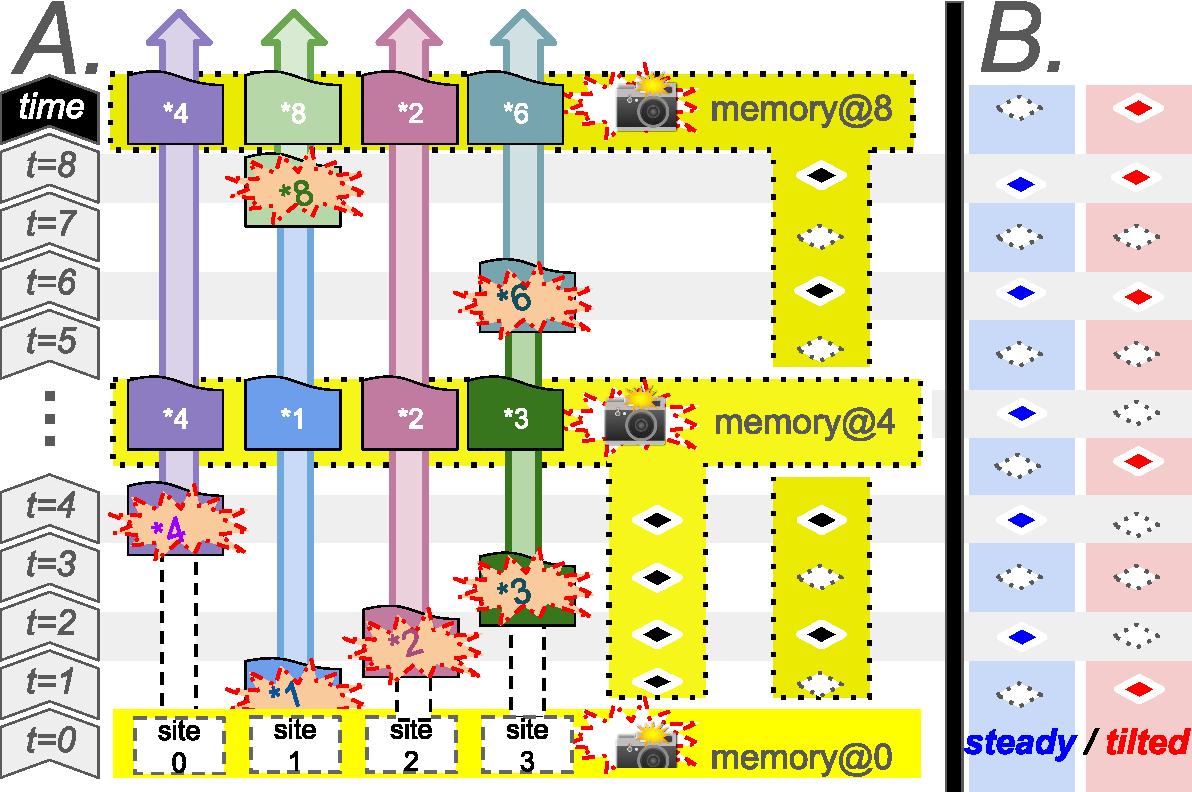
\includegraphics[width=\linewidth]{img/hsurf-schematic.pdf}
\centering
\caption{Panel A shows update sequence on a four-site HStrat curation space-time memory under steady policy. Panel B contrasts steady policy with tilted policy, which prioritizes recent data.}
\label{fig:hsurf-schematic}
\end{wrapfigure}


Instead of being maintained within a sorted list, lineage checkpoint markers are stored in a flat buffer.
This couples curation --- adding a checkpoint implicitly removes the checkpoint it overwrites.
The indexing scheme can be computed in $\mathcal{O(1)}$ time with respect to the size of the buffer and to the number of generaitons elapsed.

This has two components: a generation counter and the checkpoint marker buffer.
